\graphicspath{{./}{./figures/}{./figures/spiegelib/}}

\chapter{Inverse Synthesis}

\section{Goals}
\begin{enumerate}
    \item Main contributions: spiegelib software, initial experiments using Dexed.
    \item Goal is to explore some of the main recent approaches to inverse synthesis and compare them in the task of finding parameters to match a target sound
    \item Expand on the experimental research -- provide a bit more background on the specific methods that we are trying to emulate. Specifically: the genetic algorithm approaches and the deep learning approaches.
    \item Identify some of the challenges faced with this approach: rendering from VSTs is slow. Recent techniques SPSA could allow for VSTs to be inserted directly into the pipeline. Leads us to an area for future work: torchsynth
\end{enumerate}

Will have given a bit of a history by this point in the background -- something similar to Brecht's paper, but for automatic synthesizer programming. Here we want to focus on the main techniques that we want to use.

\section{Plan}
\begin{enumerate}
    \item This chapter explores the inverse synthesis problem. This is based on work I completed under the supervision of my supervisors and was published at AES ...
    \item Contributes SpiegeLib software and demonstrates the steps of conducting an inverse synthesis experiment through some experiments.
    \item Software in Inverse Synthesis -- overview the available software. Give some motivation based on reproducible research. Maybe add a figure that outlines the experimental process and how each of the library components fit together to help with this.
    \item SpiegeLib
    \item Experiment -- Go into more detail on the specific algorithms and methods that are being used here. Can give some code detail as well if that would be helpful.
    \item Evaluation -- How are the results evaluated and list the results
    \item Conclusion
\end{enumerate}

\section{Introduction}
The use of sound synthesizers in the fields of music composition, production, and performance is widespread, but the task of programming a synthesizer is complex and requires a thorough understanding of technical details. It is not uncommon for a software synthesizer to have 30+ parameters displayed on a user interface (UI) and labelled using technical names \cite{rasmussen2018evaluating}. Manually programming sounds using such a large set of parameters is a daunting task. Synthesizer programming is further complicated by the fact that modifications to parameters are often not intuitively reflected in the end sonic result. This disconnect can be disruptive to the creative process. Automatic synthesizer programming (ASP) is the field of research focused on addressing these challenges in programming synthesizers.

 Early ASP research emerged in the late 1970s with work that focused on the use of analytic methods to estimate the parameters for frequency modulation (FM) synthesis \cite{justice1979analytic}. That work was an example of synthesizer sound matching in which a system estimates synthesizer parameters to replicate a target sound. Since then a large volume of work on synthesizer sound matching has been published and has explored a variety of synthesis techniques and algorithmic methods. One popular approach is the use of evolutionary algorithms \cite{horner1993machine, mitchell2007evolutionary, yee2007evolving, yee2008synthbot, heise2009automatic, roth2011comparison, tatar2016automatic, smith2017play}. More recently, deep learning techniques have been explored \cite{yee2018automatic, barkan2019inversynth, esling2020flow}. Other methods that have been studied include semantic descriptions \cite{ethington1994seawave, johnson2006timbre, krekovic2016algorithm}, interactive methods \cite{johnson1999exploring, dahlstedt2001creating, yee2016use}, and sound matching with vocal imitations \cite{mcartwright2014, zhang2018visualization}.
 
 A recent user study conducted by Krekovi{\'c} et al. confirmed the desire among synthesizer users for improved means of working with their synthesizers \cite{krekovic2019insights}. 
 %Users identified approaches they felt would be particularly beneficial, which included automatic sound matching and improvements to user interface design. 
 While recent research has produced promising results, automatically programming a modern software synthesizer still presents challenges. Current evolutionary techniques face issues including time complexity \cite{tatar2016automatic}, while recent deep learning approaches have challenges in consistently producing accurate reproductions \cite{yee2018automatic}. The desires expressed by the users in Krekovi{\'c} et al.'s study, coupled with the need for further research and improvement noted in the existing body of work, point to the need for further development in ASP.
 
 The work presented here attempts to continue this development, and promote collaboration and reproducibility in ASP research through the introduction of \mintinline{python}{spiegelib}, an open-source library written in the Python programming language. Vandewalle et al. argue that reproducibility in computational science research increases the impact of a work and they provide a framework for evaluating the quality of reproducibility \cite{vandewalle2009reproducible}. The aim of \mintinline{python}{spiegelib} is to provide a platform for researchers of automatic synthesizer programming to develop, test, and share implementations in a way that promotes reproducibility at the highest level. \mintinline{python}{spiegelib} stands for Synthesizer Programming with Intelligent Exploration, Generation, and Evaluation Library. The name \mintinline{python}{spiegelib} was chosen to pay homage to Laurie Spiegel, an early pioneer in electronic music composition. Laurie Spiegel is known for utilizing synthesizers and software to automate certain aspects of the music composition process. Her philosophy for using technology in music serves as a motivation for the \mintinline{python}{spiegelib} software library: "I automate whatever can be automated to be freer to focus on those aspects of music that can't be automated. The challenge is to figure out which is which." \cite{hinkle2006women}
 
 The remainder of this paper is structured as follows: Section \ref{sec:2} presents a survey of related work to provide background for the algorithmic techniques included in \mintinline{python}{spiegelib} as well as an overview of available open-access ASP software, Section \ref{sec:3} provides an overview of the \mintinline{python}{spiegelib} software library. An example case illustrating the use of \mintinline{python}{spiegelib} in a research context is presented in Section \ref{sec:4}.

\section{Related Work}\label{sec:2}
This section provides a brief summary of the main algorithmic methodologies that have been used in previous ASP research, namely, optimization and deep learning techniques. Other methods that have been used in ASP research that are beyond the scope of this paper include  include fuzzy logic \cite{mitchell2005frequency, hamadicharef2012intelligent}, linear coding \cite{mintz2007toward}, and query approaches \cite{mcartwright2014}. An  informal survey of open-access software that supports reproducibility is also included at the end of the section.

\subsection{Optimization}
The optimization approach was first introduced in 1993 with Horner et al.'s work on sound matching for FM synthesis using genetic algorithms \cite{horner1993machine}. A genetic algorithm (GA) is a method for solving an optimization problem using techniques based on the principles of Darwinian evolution, and is part of a broader class of evolutionary algorithms \cite{whitley1994genetic}. In a GA, a potential solution (an individual) is represented as an array of bits. An initial set of individuals is randomly generated, and then iteratively evolved using biologically inspired processes including selection, breeding, and mutation. Individuals are ranked using an evaluation function that measures the $fitness$ of a given solution. The objective of a GA is to minimize that value (or maximize it, depending on the problem definition). The best candidates are selected for further evolution until either an optimal solution is found or a set number of evolutions has been completed.

In the case of sound matching, the \textit{fitness} of a potential solution is determined by measuring the error between a target sound and a candidate. Typically, an audio transform or audio feature extraction is performed prior to calculating \textit{fitness}. The first works on synthesizer sound matching with GAs used the Short Time Fourier Transform (STFT) in the evaluation function \cite{horner1993machine, horner1995wavetable}. Mel-frequency Cepstral Coefficients (MFCCs), an audio representation using a non-linear frequency scaling that is more relevant to human hearing, have also been used \cite{yee2008synthbot, roth2011comparison, macret2014automatic, smith2017play}. Tatar et al. introduced the use of a multi-objective GA for synthesizer sound matching that used three different methods for calculating $fitness$ values: the STFT, Fast Fourier Transform (FFT), and signal envelope \cite{tatar2016automatic}. Alternatives to GAs that have been used for sound matching include Particle Swarm Optimization (PSO) \cite{heise2009automatic} and Hill-Climbing \cite{roth2011comparison, luke2019stochastic}.

Researchers have also used Interactive Genetic Algorithms (IGAs) that allow users to interactively hear and rate potential synthesizer patches \cite{johnson1999exploring, dahlstedt2001creating, yee2016use}. In contrast to the sound matching case, the evaluation function in an IGA relies on user feedback during each iteration as opposed to measuring error between a candidate and a target. 

Automatic programming using semantic sound descriptions has also been explored, and is a further methodology that has used GAs \cite{krekovic2016algorithm}.

\subsection{Deep Learning}
Deep learning is subset of machine learning that utilizes artificial neural networks to learn patterns in data and make predictions based on those patterns \cite{lecun2015deep}. Deep learning architectures contain multiple layers comprised of simple non-linear modules. Through iterative training, the layers are able to extract features from raw input data and learn intricate patterns in high-dimensional data. These multi-layer architectures have enabled deep learning models to excel at complex tasks including image recognition, speech recognition, and music related tasks such as audio source separation \cite{spleeter2019}.

In the context of an ASP sound matching experiment, a deep learning model accepts an audio signal as input and predicts synthesizer parameter settings to replicate that audio signal. Audio signals are often preprocessed using audio feature extraction or an audio transform. Models are trained using a large set of example sounds generated from a synthesizer and use the parameter settings that generated a particular sound as the ground truth. During training, the error between predicted parameter settings and the actual parameter settings (the ground truth) are used to evaluate how well the model is learning and to iteratively update variables within the model to improve performance. 

Several researchers have explored the use of deep learning for ASP. Yee-King et al. reviewed several deep learning architectures for FM synthesizer sound matcing [11]. In their work, they compared multi-layer perceptron (MLP), Long Short Term Memory (LSTM), and LSTM++ networks. Barkan et al. explored sound matching using convolutional neural networks (CNNs) [12]. They framed the problem as an image classification task and used the STFT to create spectrogram images of target sounds to use as input to the CNNs. Esling et al. recently presented a novel application called $FlowSynth$ that uses a generative model based on Variational Auto-Encoders and Normalizing Flows [13]. In addition to performing well on sound matching tasks, they also showed that their approach supported novel interactions including macro-control of synthesizer parameters.

\subsection{Software in ASP Research}
 In Vandewalle et al.'s paper on reproducibility in computational sciences, they advocate providing other researchers with "all the information (code, data, schemes, etc.) that was used to produce the presented results"\cite{vandewalle2009reproducible}. Several authors of ASP research have started to make their work open-access with source code available online. 
 
 Martin Roth and Matthew Yee-King developed $JVstHost$, a Java-based Virtural Studio Technology (VST) plugin host that was published by Matthew Yee-King \cite{yee2011automatic} and was a component of $SynthBot$ \cite{yee2008synthbot}. However, the code for $SynthBot$ itself was not released. Matthew Yee-King also shared the source code for $EvoSynth$, an application for interactive synthesizer patch exploration \cite{yee2016use}. A version of $EvoSynth$ is hosted online allowing for immediate experimentation\footnote{\url{http://www.yeeking.net/evosynth/}}. Krekovi{\'c} et al. released source code for their $MightyKnob$ system \cite{krekovic2016algorithm}. Esling et al. released open-source code and a Max4Live\footnote{\url{https://www.ableton.com/en/live/max-for-live/}} application for $FlowSynth$ \cite{esling2020flow}. Yee-King et al. recently took initial steps towards a software framework for ASP research with the release of source code that provides functionality for generating research datasets and a set of algorithms for parameter estimation \cite{yee2018automatic}. Along with that work they released the $RenderMan$\footnote{\url{https://github.com/fedden/RenderMan}} library for programmatically interacting with VST synthesizers using the Python programming language.
 
 \mintinline{python}{spiegelib} builds upon this work with the goal of supporting and encouraging reproducibility within the ASP research community. \mintinline{python}{spiegelib} is inspired by the steps that Yee-King et al. took towards creating a software library for ASP research and extends that work with the inclusion of: an object-oriented API, base classes for customization, more robust evolutionary techniques, basic subjective evaluation, complete documentation, and packaging and delivery. It provides a framework for authors to share implementations in an open-access way that allows other researchers to quickly recreate results using a clearly documented set of freely-available tools.
 
% Updated table if necassary
%\begin{table*}[t]
%\centering\small
%\begin{threeparttable}
%	\caption{Algorithms currently implemented as classes in \mintinline{python}{spiegelib}}
%	\label{table:spiegel_algorithms}
%	\begin{tabular}{|c|c|c|c|}
%	\hline
%	\multicolumn{4}{|c|}{\textbf{Algorithms in \mintinline{python}{spiegelib}}} \\
%	\hline
%	\hline
%	\textbf{Feature Extraction} & \textbf{Deep Learning Estimators} & \textbf{Optimization Estimators} & \textbf{Evaluation} \\
%	\hline
%	FFT 		& MLP \cite{yee2018automatic} 		& Basic GA  	& MFCC Evaluation \\
%	STFT 		& LSTM \cite{yee2018automatic} 		& NSGA III \cite{tatar2016automatic} & Basic Subjective \\\cline{3-4}
%	MFCC		& LSTM++ \cite{yee2018automatic} \\
%	Spectral\tnote{1}	& Conv6 \cite{barkan2019inversynth} \\\cline{1-2}
%	\end{tabular}
%	\begin{tablenotes}[para, flushleft]
%			\footnotesize
%			\item[1] Spectral bandwidth, centroid, contrast, flatness, and rolloff.
%	\end{tablenotes}
%\end{threeparttable}
%\end{table*}

\begin{table*}[t]
\centering\small
\begin{threeparttable}
	\caption{Algorithms currently implemented as classes in \mintinline{python}{spiegelib}}
	\label{table:spiegel_algorithms}
	\begin{tabular}{|c|c|c|}
	\hline
	\multicolumn{3}{|c|}{\textbf{Algorithms in \mintinline{python}{spiegelib}}} \\
	\hline
	\hline
	\textbf{Feature Extraction} & \textbf{Deep Learning Estimators} & \textbf{Optimization Estimators} \\
	\hline
	FFT 		& MLP \cite{yee2018automatic} 		& Basic GA   			\\
	STFT 		& LSTM \cite{yee2018automatic} 		& NSGA III \cite{tatar2016automatic}				\\\cline{3-3}
	MFCC		& LSTM++ \cite{yee2018automatic} 	& \textbf{Objective Evaluation} 	\\\cline{3-3}
	Spectral\tnote{1}	& Conv6 \cite{barkan2019inversynth} 	& MFCC Evaluation 		\\
	\hline
	\end{tabular}
	\begin{tablenotes}[para, flushleft]
			\footnotesize
			\item[1] Spectral bandwidth, centroid, contrast, flatness, and rolloff.
	\end{tablenotes}
\end{threeparttable}
\end{table*}
 
\section{Design of SpiegeLib}\label{sec:3}
\mintinline{python}{spiegelib} is designed to be as extensible as possible to allow researchers to develop and test new implementations of components for conducting ASP research. Base classes with functionality for interacting with software synthesizers, audio feature extraction, parameter estimation, and evaluation provide an API to support development of custom implementations that will work with other components of the library. A number of utility classes are also provided for handling audio signals, generating datasets, and running experiments.

 \mintinline{python}{spiegelib} is written in the Python programming language and utilizes Python packages common in research including \mintinline{python}{numpy}, \mintinline{python}{scipy}, \mintinline{python}{tensorflow}, and \mintinline{python}{librosa}. \mintinline{python}{spiegelib} itself is a python package and is available through the Python Package Index (PyPI) with pip\footnote{\url{https://pypi.org/}}. All dependencies, except for \mintinline{python}{librenderman}, are python packages available through the PyPI and will be automatically installed by pip. For more information on installation, system requirements, and detailed library documentation, please refer to the  online documentation.\footnote{\url{https://spiegelib.github.io/spiegelib/}}
 
 A summary of the currently implemented algorithms is shown in table \ref{table:spiegel_algorithms}. A brief overview of these components and the main classes and functionalities of \mintinline{python}{spiegelib} is provided in the following sections.
 
\subsection{AudioBuffer}
The \mintinline{python}{AudioBuffer} class is used to pass audio signal signals throughout the library. It holds an array of audio samples and sample rate information. Methods of the \mintinline{python}{AudioBuffer} class provide functionality for loading audio from a variety of file formats, resampling, normalizing, time segmenting, plotting spectrograms, and saving audio as WAV files.

\subsection{Synthesizers}
The \mintinline{python}{SynthBase} class is an abstract base class that provides an interface for creating programmatic interactions with software synthesizers. \mintinline{python}{SynthBase} stores information and contains methods required for interaction with other components in \mintinline{python}{spiegelib}, including getting parameter lists, setting and getting patch configurations, overriding/freezing parameters, triggering audio rendering using MIDI notes, getting audio samples as \mintinline{python}{AudioBuffer}s, and requesting randomized patch settings. All patch settings are stored as a list of parameter tuples which contain the parameter number and parameter value. All parameter values are expected to be floating point numbers in the range [0.0, 1.0]. No requirement is made on how underlying synthesis engines are implemented, however, inheriting classes must provide parameter descriptions in a class attribute during construction and must provide implementations for four abstract class methods related to loading patches, randomizing patches, rendering audio, and returning an \mintinline{python}{AudioBuffer} of rendered audio.

%
% \mintinline{python}{load_patch()}, \mintinline{python}{randomize_patch()}, \mintinline{python}{render_patch()}, and \mintinline{python}{get_audio()}.

\mintinline{python}{SynthVST} is an implementation of \mintinline{python}{SynthBase} and provides an interface for interacting with VST synthesizers. \mintinline{python}{SynthVST} is a wrapper for the $RenderMan$ Python library developed by Leon Fedden in conjunction with research by Yee-King et al. \cite{yee2018automatic}.

\subsection{Audio Feature Extraction}
The abstract base class \mintinline{python}{FeaturesBase} provides an interface for audio feature extraction tasks. 
The \mintinline{python}{getFeatures()} abstract method must be overridden in inheriting classes and is where feature extraction algorithms are run.  \mintinline{python}{FeatureBase} also includes functionality for normalizing results from feature extraction. By default, data is normalized by removing the mean and scaling to unit variance. Settings for normalization can be saved from a set of data, reloaded, and applied to new feature extraction results to ensure that normalization is carried out using the same parameters. Currently, implemented feature extraction classes utilize the \mintinline{python}{librosa} library \cite{mcfee2015librosa} and include Mel Frequency Cepstral Coefficients (\mintinline{python}{MFCC}), Short Time Fourier Transform (\mintinline{python}{STFT}), Fast Fourier Transform (\mintinline{python}{FFT}), and a set of time summarized spectral features (\mintinline{python}{SpectralSummarized}).

\subsection{Estimators}
All parameter estimation classes implement the \mintinline{python}{EstimatorBase} abstract base class. \mintinline{python}{EstimatorBase} is a minimal base class with one abstract method, \mintinline{python}{predict()}, that has an optional input argument. Implementations of estimators are split into deep learning approaches and other approaches including evolutionary algorithms.  The included algorithms do not represent a comprehensive set of methods for ASP research but are meant to cover common methods informed by previous work. Six estimators are currently implemented and the authors plan to add 5 more in the near future: a hill climbing optimizer \cite{yee2018automatic}, a particle swarm optimizer \cite{heise2009automatic}, additional configurations of 2D CNNs \cite{barkan2019inversynth}, a 1D CNN for raw audio input \cite{barkan2019inversynth}, and a recent generative approach \cite{esling2020flow}. The authors hope that other researchers will add their new algorithms to the library as well.

\subsubsection{Deep Learning Estimators}
All deep learning models are implementations of the \mintinline{python}{TFEstimatorBase} abstract base class which utilizes the \mintinline{python}{tensorflow}\footnote{\url{https://www.tensorflow.org}} and \mintinline{python}{keras}\footnote{\url{https://www.tensorflow.org/guide/keras}} machine learning libraries. \mintinline{python}{TFEstimatorBase} implements \mintinline{python}{EstimatorBase} and provides wrapper functions for setting up data for training and validation, training models, running predictions, and saving and loading model weights. While these methods are designed to help in handling of data typical to a synthesizer parameter estimation problem, all methods for a \mintinline{python}{tf.keras.Model} can be accessed directly from the \mintinline{python}{model} class member. Classes that inherit from \mintinline{python}{TFEstimatorBase} define models in an implementation of the \mintinline{python}{buildModel()} method which is automatically called during construction in the base class. This allows new models to be quickly designed, switched out, and compared with minimal effort.

Currently, implementations for a Multi-Layer Perceptron (\mintinline{python}{MLP}), Long Short Term Memory (\mintinline{python}{LSTM}), Bi-directional Long Short Term Memory with Highway Layers (\mintinline{python}{HwyBLSTM}), and a convolution network with 6-layers (\mintinline{python}{Conv6}) are included. An example code listing of sound matching using a trained LSTM model is shown in figure \ref{fig:lstm_code}.

To save training and validation progress, the \mintinline{python}{TFEpochLogger} class can be passed in as a callback during model training. \mintinline{python}{TFEpochLogger} stores training accuracy and loss, and validation accuracy and loss over training epochs in a dictionary object which can be plotted after training.

%Example code listing
\begin{figure}[t]
\centering
\caption{Example of \mintinline{python}{spiegelib} performing a sound match from a target WAV file on a VST synthesizer. A pre-trained LSTM deep learning model is used with MFCC input.}
\footnotesize
\begin{minted}{python}
import spiegelib as spgl
import spiegelib.estimator.TFEstimatorBase

# Load VST and set parameters from JSON file
synth = spgl.synth.SynthVST('./Dexed.vst')
synth.load_state('./dexed_simple_fm.json')

# MFCC Audio Feature Extractor
ftrs = spgl.features.MFCC(normalize=True)

# Load saved normalization parameters
ftrs.load_normalizers('./normalizers.pkl')

# Load LSTM model from saved model file
lstm = TFEstimatorBase.load('./fm_lstm.h5')

matcher = spgl.SoundMatch(synth, lstm, ftrs)

target = spgl.AudioBuffer('./target.wav')
output = matcher.match(target)
output.save('./lstm_predicted_audio.wav')
\end{minted}
\label{fig:lstm_code}
\end{figure} 

\subsubsection{Optimization Estimators}
Two optimization estimators are currently implemented and utilize the DEAP python library \cite{fortin2012deap}. A basic GA (\mintinline{python}{BasicGA}) is included as well as a multi-objective non-dominated sorting genetic algorithm III (\mintinline{python}{NSGA3}). Both GAs require feature extraction objects, or a list of feature extraction objects in the case of the multi-objective algorithm, which are used in the GA evaluation function. 

\subsection{Datasets}
The \mintinline{python}{DatasetGenerator} class provides functionality for creating datasets of audio samples, feature vectors, and associated parameter settings from a synthesizer. An implementation of \mintinline{python}{SynthBase} and \mintinline{python}{FeaturesBase} are passed in as arguments to the \mintinline{python}{DatasetGenerator} constructor. To generate a dataset, random patches for the synthesizer are created and feature extraction is performed on the resulting audio. In this way, datasets for training and validating deep learning models, as well as datasets for evaluating sound matching experiments can be automatically generated. 
%The term contrived in the context of ASP research refers to the use of audio samples produced by the synthesizer being studied as a target for sound matching \cite{justice1979analytic}. The benefit of using a contrived sound for evaluation is that it minimizes the uncertainty regarding whether the synthesizer in question is capable of producing the target sound. 
External datasets can also be used within \mintinline{python}{spiegelib} and the \mintinline{python}{AudioBuffer} class provides support for loading folders of audio samples for processing.

\subsection{Evaluation}
Objective evaluation of results can be carried out by measuring error between audio samples. \mintinline{python}{EvaluationBase} is an abstract base class for calculating evaluation metrics on a set of target and prediction data. A list of target values and lists of predictions for each target are passed into the constructor. \mintinline{python}{EvaluationBase} provides functionality for calculating statistics on results, saving results as a JSON file, plotting results in histograms, and calculating metrics including mean absolute error, mean squared error, euclidian distance, and manhattan distance. Inheriting classes must implement the \mintinline{python}{evaluate_target()} method which is called for each target and associated estimations and is expected to return a dictionary of metrics for each estimation. The \mintinline{python}{MFCCEval} class implements \mintinline{python}{EvaluationBase} and calculates metrics on MFCC vectors for targets and estimations.

Functionality for conducting subjective evaluation of results is provided in the \mintinline{python}{BasicSubjective} class. This class accepts a set of audio files and runs a locally hosted server that generates a simple web interface for listening to and ranking audio files in terms of similarity or preference. For sound matching experiments, audio targets can be passed in along with a set of predictions for each target, and a sound similarity test will be generated with options for randomizing the ordering of targets and predictions. Results can then be saved as a JSON file.

\section{Example Case}\label{sec:4}
\subsection{Dexed: FM Sound Matching}
To illustrate the use of \mintinline{python}{spiegelib} in the context of an ASP sound matching experiment, we present an example study that compares six different parameter estimators acting on $Dexed$\footnote{\url{https://asb2m10.github.io/dexed/}}, a VST software emulation of the Yamaha DX7 FM synthesizer. The methodology used for this experiment is modelled after Yee-King et al.'s study on deep learning for automatic synthesizer programming \cite{yee2018automatic}, but with a simplified synthesizer configuration and a unique set of estimators. In alignment with Vandewalle et al.'s criteria for reproducible research, implementation details, code, and datasets are all available on the \mintinline{python}{spiegelib} online documentation.\footnote{\url{https://spiegelib.github.io/spiegelib/examples/fm_sound_match.html}}

The first step is defining the synthesizer setup and creating data for training deep learning models. $Dexed$ has 155 parameters controllable through the \mintinline{python}{SynthVST} class. A subset of nine of these parameters were used in this experiment to turn $Dexed$ into a simple two-oscillator FM synthesizer. The \mintinline{python}{SynthVST} class provides methods for overriding and freezing parameters as well as saving and loading parameter settings as JSON files.

The \mintinline{python}{DatasetGenerator} class was then used to create datasets for deep learning training. All deep learning models, except for the CNN, used a 13-band MFCC calculated with a frame size of 2048 samples and a hop size of 1024 samples. The input of the CNN was the magnitude spectrum from a STFT, calculated using an FFT with 512 bins and a hop size of 256 samples. Using an instance of \mintinline{python}{DatasetGenerator}, 50,000 training examples and 10,000 validation examples were generated by randomly sampling the nine parameters from $Dexed$. Resulting feature vectors were normalized by removing the mean and scaling to unit variance using methods within the \mintinline{python}{FeatureBase} base class. Datasets and settings for normalization were then stored as NumPy\footnote{\url{https://numpy.org/}} files for later use.

All deep learning models are defined in classes within \mintinline{python}{spiegelib} and all inherit from \mintinline{python}{TFEstimatorBase}. Models were trained using an $Adam$ optimizer \cite{kingma2014adam}, batch sizes of 64, and used an early stopping callback which halted training if validation loss was stagnant for 10 epochs to prevent overfitting. Logging of training and validation progress was recorded using the \mintinline{python}{TFEpochLogger} class. The loss function in all models measure the RMS error between ground truth parameter settings and prediction parameter settings. 
%Plots of training and validation accuracy and loss for the LSTM++ model are shown in figure \ref{fig:lstm_bi_train}. Trained models are then saved for future use.

%\begin{figure}[]
%\begin{center}
%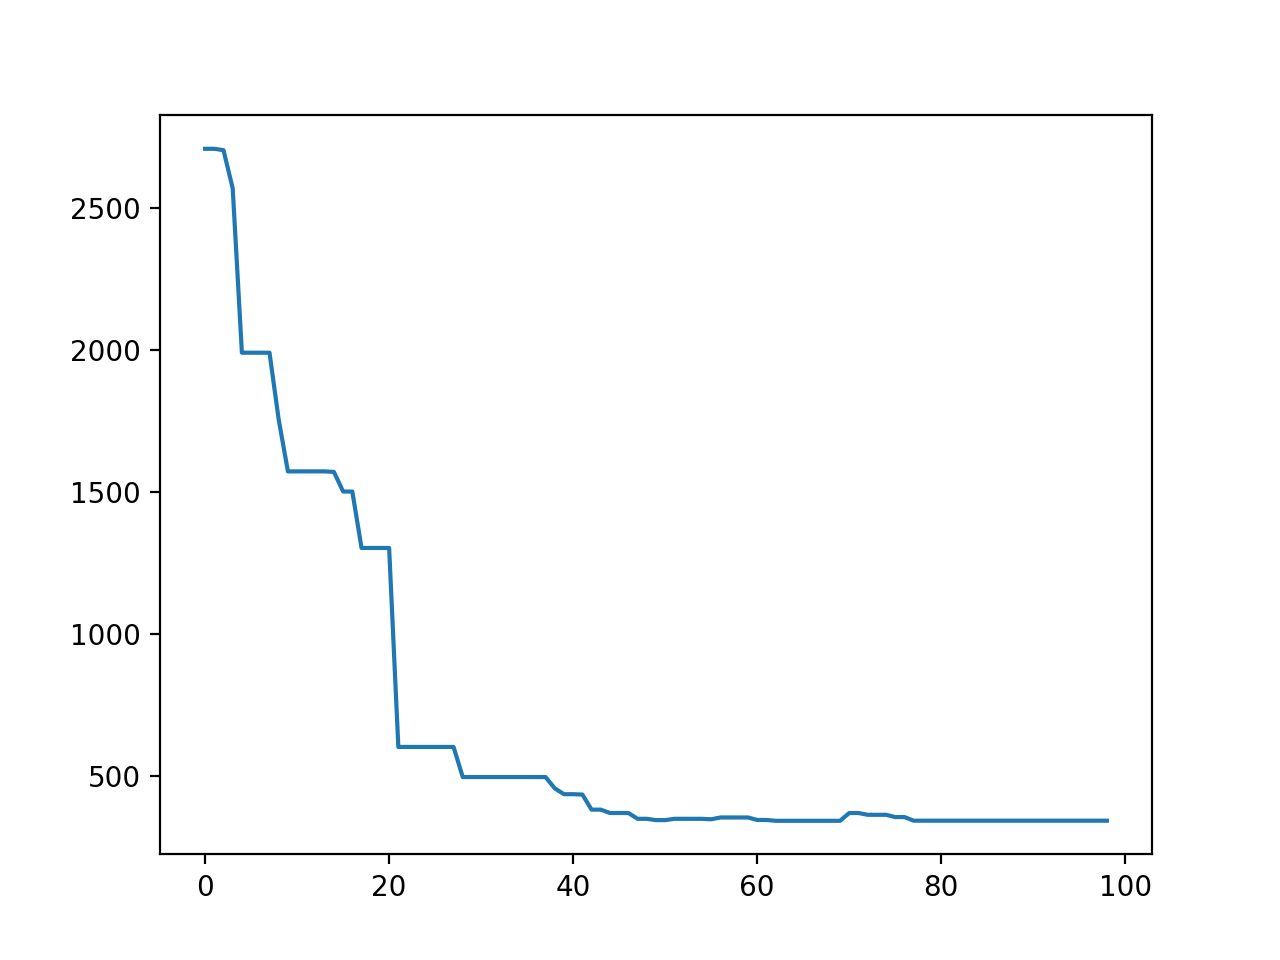
\includegraphics[width=0.95\columnwidth]{nsga_target_15_FFT.png}
%\caption{Minimum FFT MAE in the population at each generation to target sound 15 for NSGA III estimator.}
%\label{fig:nsga_fitness}
%\end{center}
%\end{figure}

Two GAs were used: a basic single-objective GA (\mintinline{python}{BasicGA}) and a multi-objective NSGA III (\mintinline{python}{NSGA3}). Evaluation functions for the GAs use audio feature extraction and measure the mean absolute error (MAE) between the target and individuals to calculate $fitness$. The \mintinline{python}{BasicGA} used a 13-band MFCC in the evaluation function and the \mintinline{python}{NSGA3} used three different extractors: a 13-band MFCC, STFT, and five spectral features. Both genetic algorithms were run for 100 generations for each sound target.

%\begin{figure}[t]
%\begin{center}
%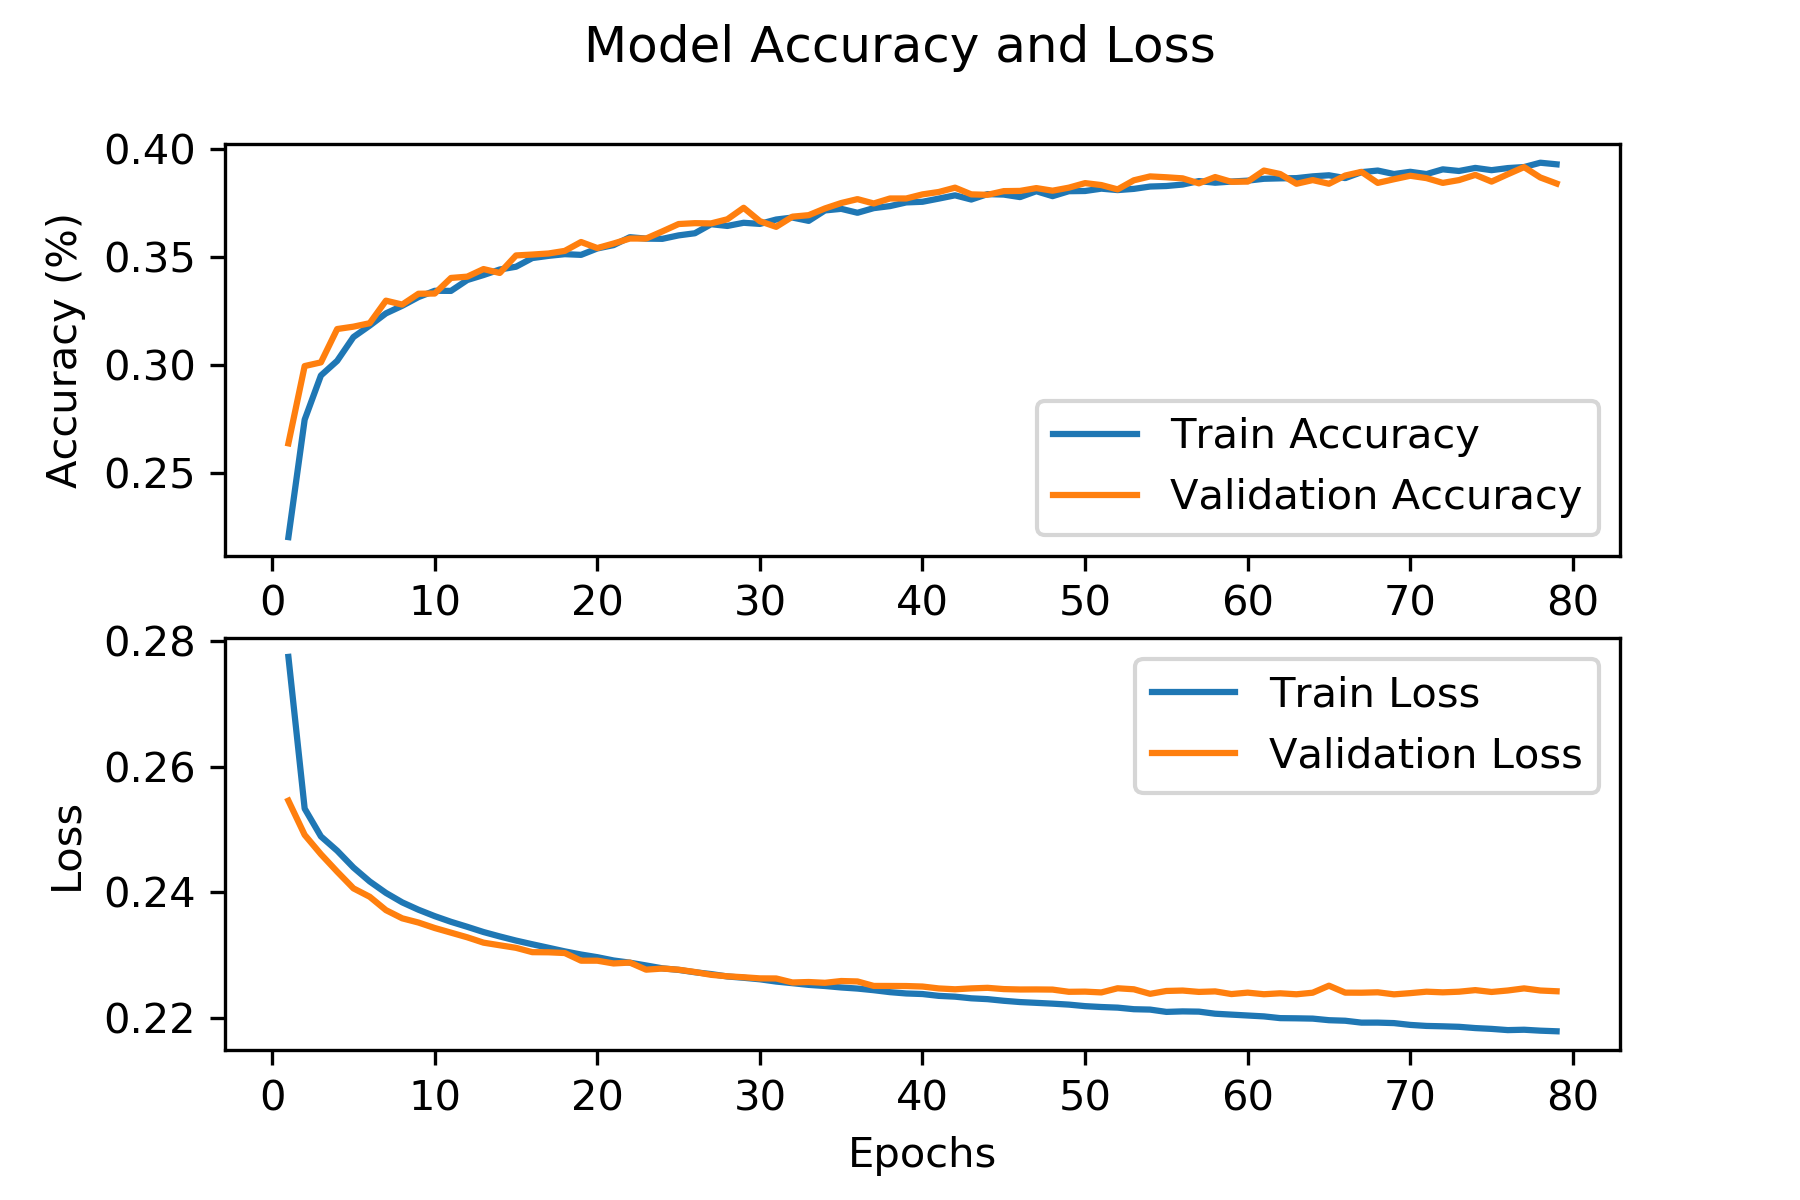
\includegraphics[width=0.95\columnwidth]{blstm_training.png}
%\caption{Traing and validation accuracy and loss over epochs for LSTM++ model training.}
%\label{fig:lstm_bi_train}
%\end{center}
%\end{figure}

An evaluation dataset containing 25 random sounds from the same nine-parameter $Dexed$ configuration was generated using the \mintinline{python}{DatasetGenerator} class. All estimators were run on each one of the 25 target sounds using the \mintinline{python}{SoundMatch} class. \mintinline{python}{SoundMatch} is a functional class that uses an estimator to predict synthesizer parameter settings for an implementation of \mintinline{python}{SynthBase} in order to match a target sound. This resulted in a set of audio files generated from $Dexed$ using the estimated parameters from each estimator run on each of the 25 target sounds. These audio files were then used for objective evaluation.

\begin{table}[t]
\centering
\caption{Results from sound matching evaluation}
\label{tbl:sound_match_eval}
\begin{threeparttable}
\begin{tabular}{l|cccc}
\toprule
$Method$ & $Mean$ & $SD$ & $Min$ & $Max$ \\
\midrule
$MLP$ & 8.55 & 6.77 & 1.92 & 34.12 \\
$CNN$ & 7.88 & 4.26 & 2.68 & 20.89 \\
$LSTM$ & 6.12 & 3.76 & 1.20 & 19.36 \\
$LSTM++$ & 4.91 & 6.50 & 2.12 & 21.51 \\
$GA$ & 2.25 & 2.58 & 0.70 & 11.17 \\
$NSGA III$ & \textbf{0.81} & \textbf{0.89} & \textbf{0.001} & \textbf{3.06} \\
\bottomrule
\end{tabular}
\begin{tablenotes}[para, flushleft]
\footnotesize
\item Values shown are calculated from the mean absolute error (MAE) calculated during MFCC evaluation. Smaller MAE values indicate more similar matches. The NSGA III estimator received the best scores, which are shown in bold font.
\end{tablenotes}
\end{threeparttable}
%\vspace{5mm}
\end{table}

\begin{figure}[t]
\begin{center}
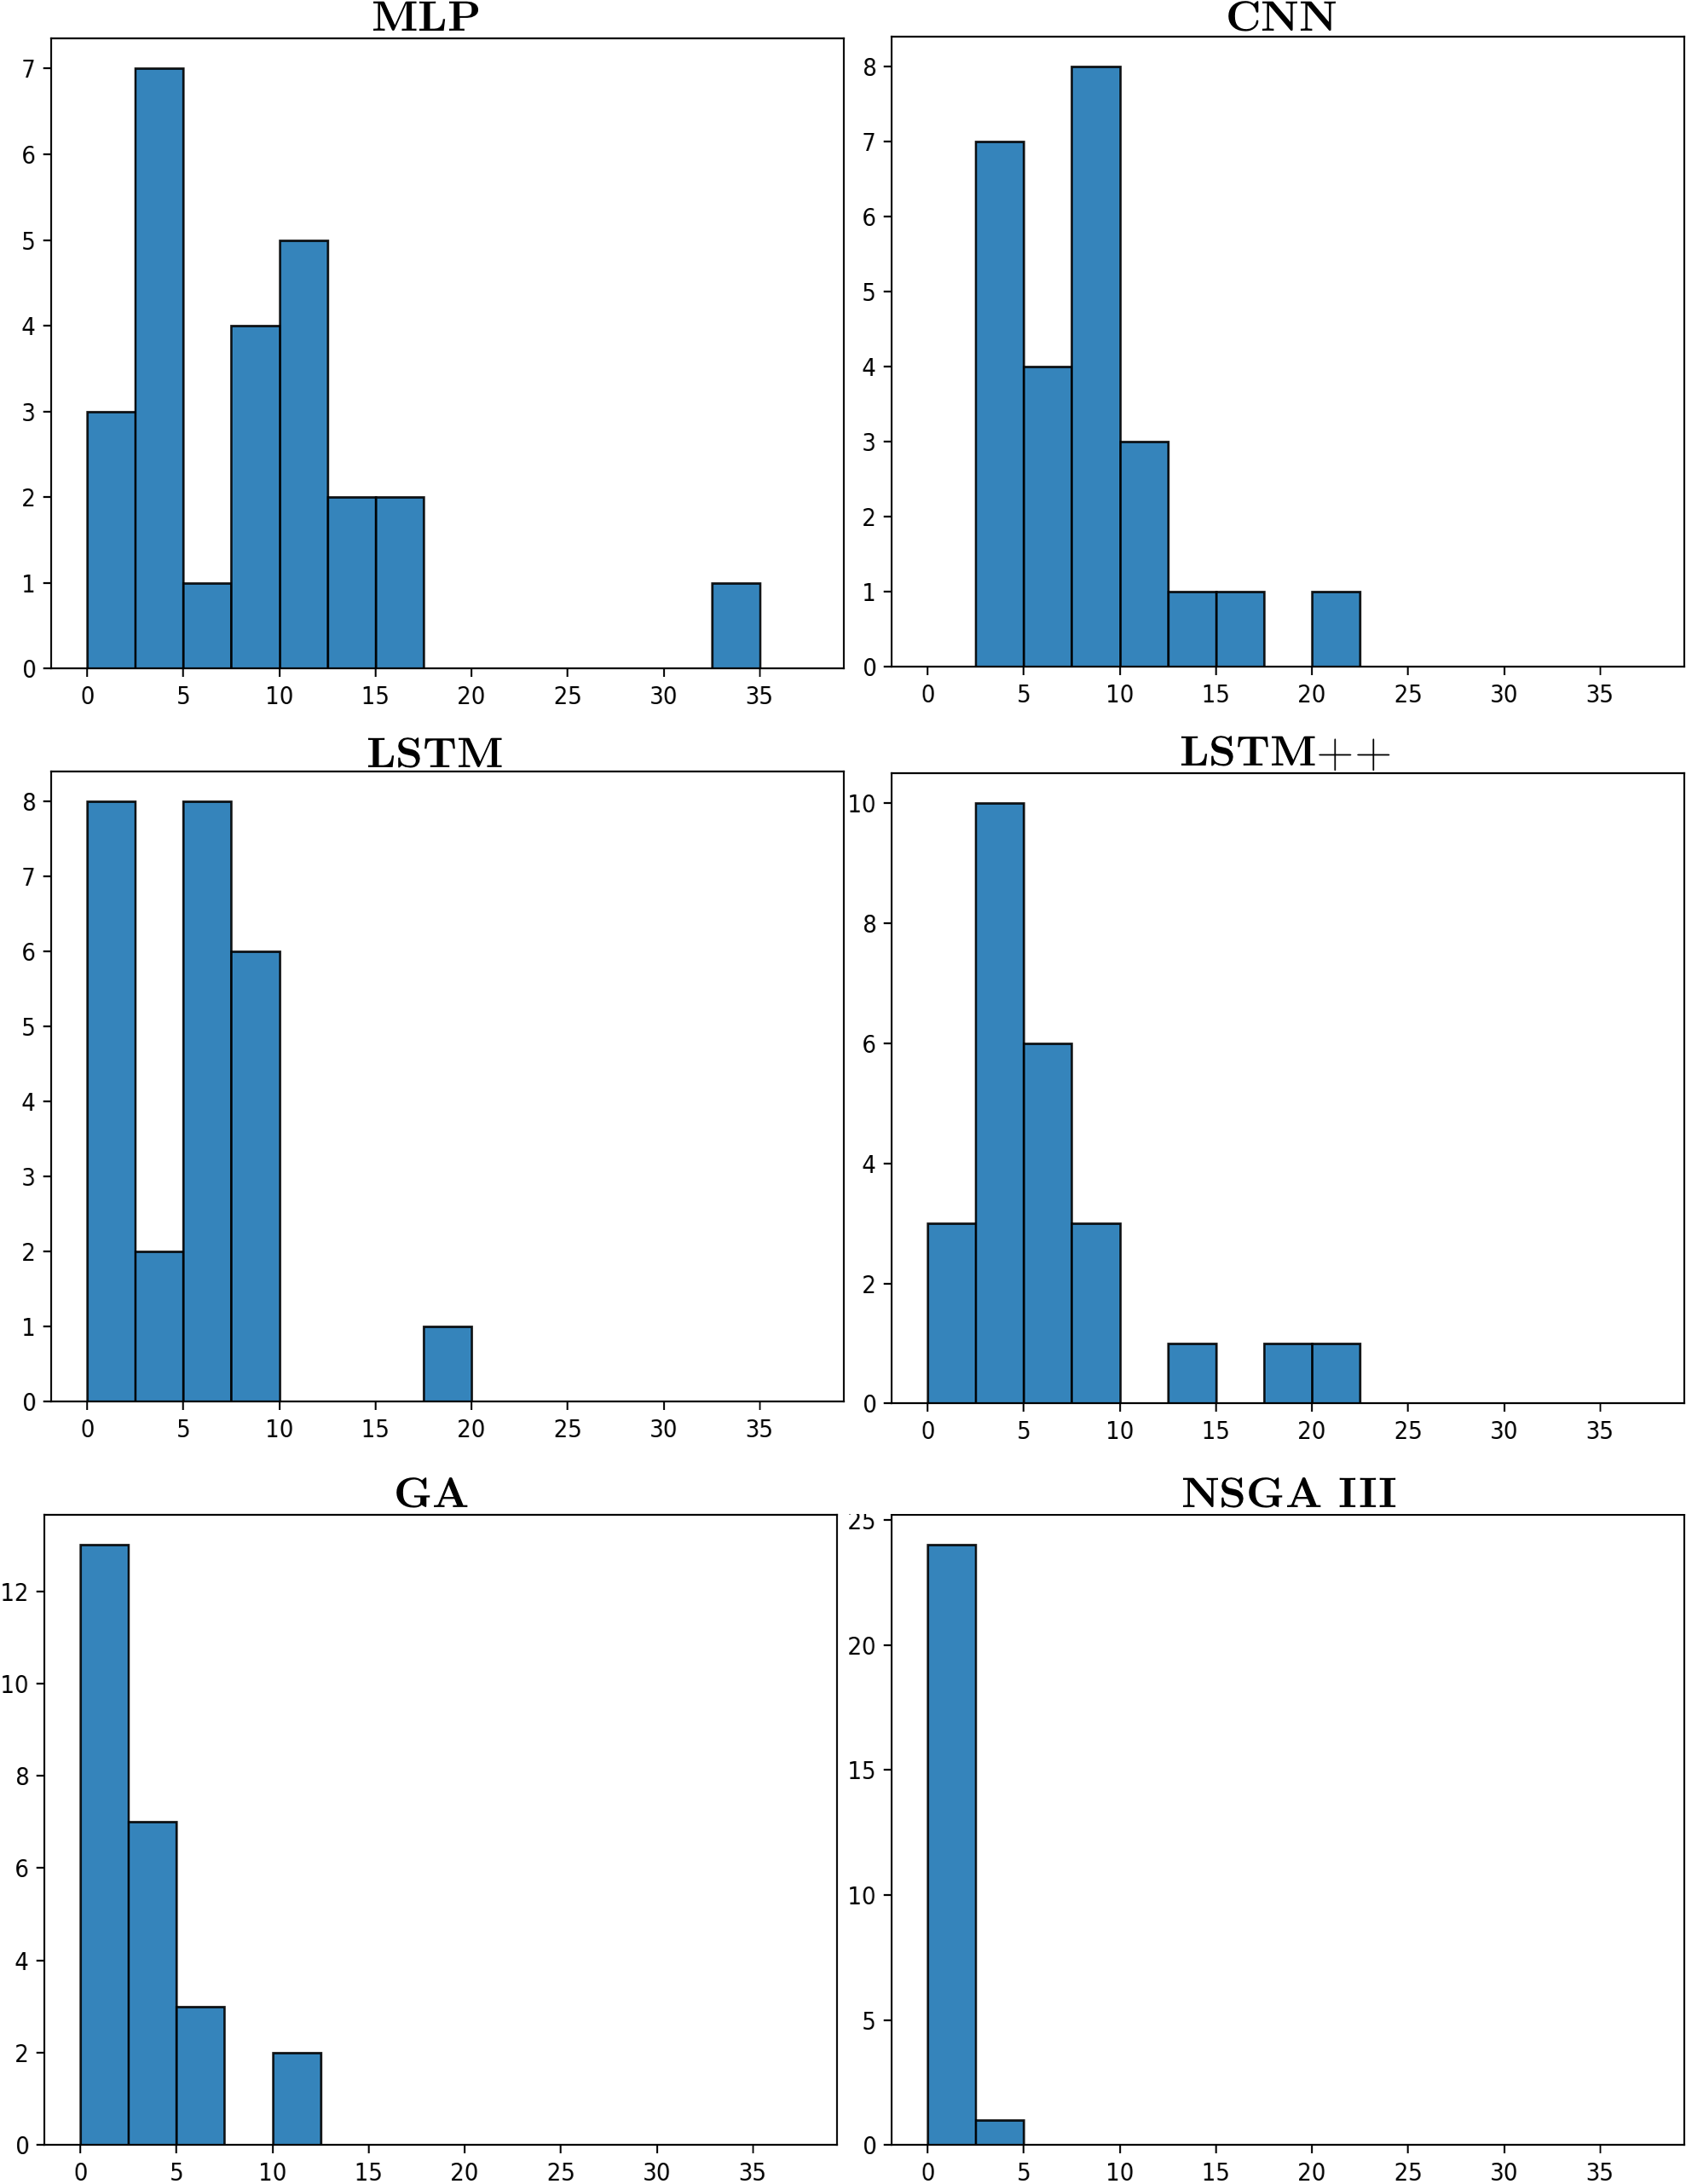
\includegraphics[width=0.75\textwidth]{hist_group_v3.png}
\caption{Histogram shows the MAE values resulting from MFCC evaluation run on a set of 25 sound targets for all estimators. Lower MAE values indicate a closer sound match.}
\label{fig:group_hist}
\end{center}
\end{figure}

\begin{figure}[t]
\begin{center}
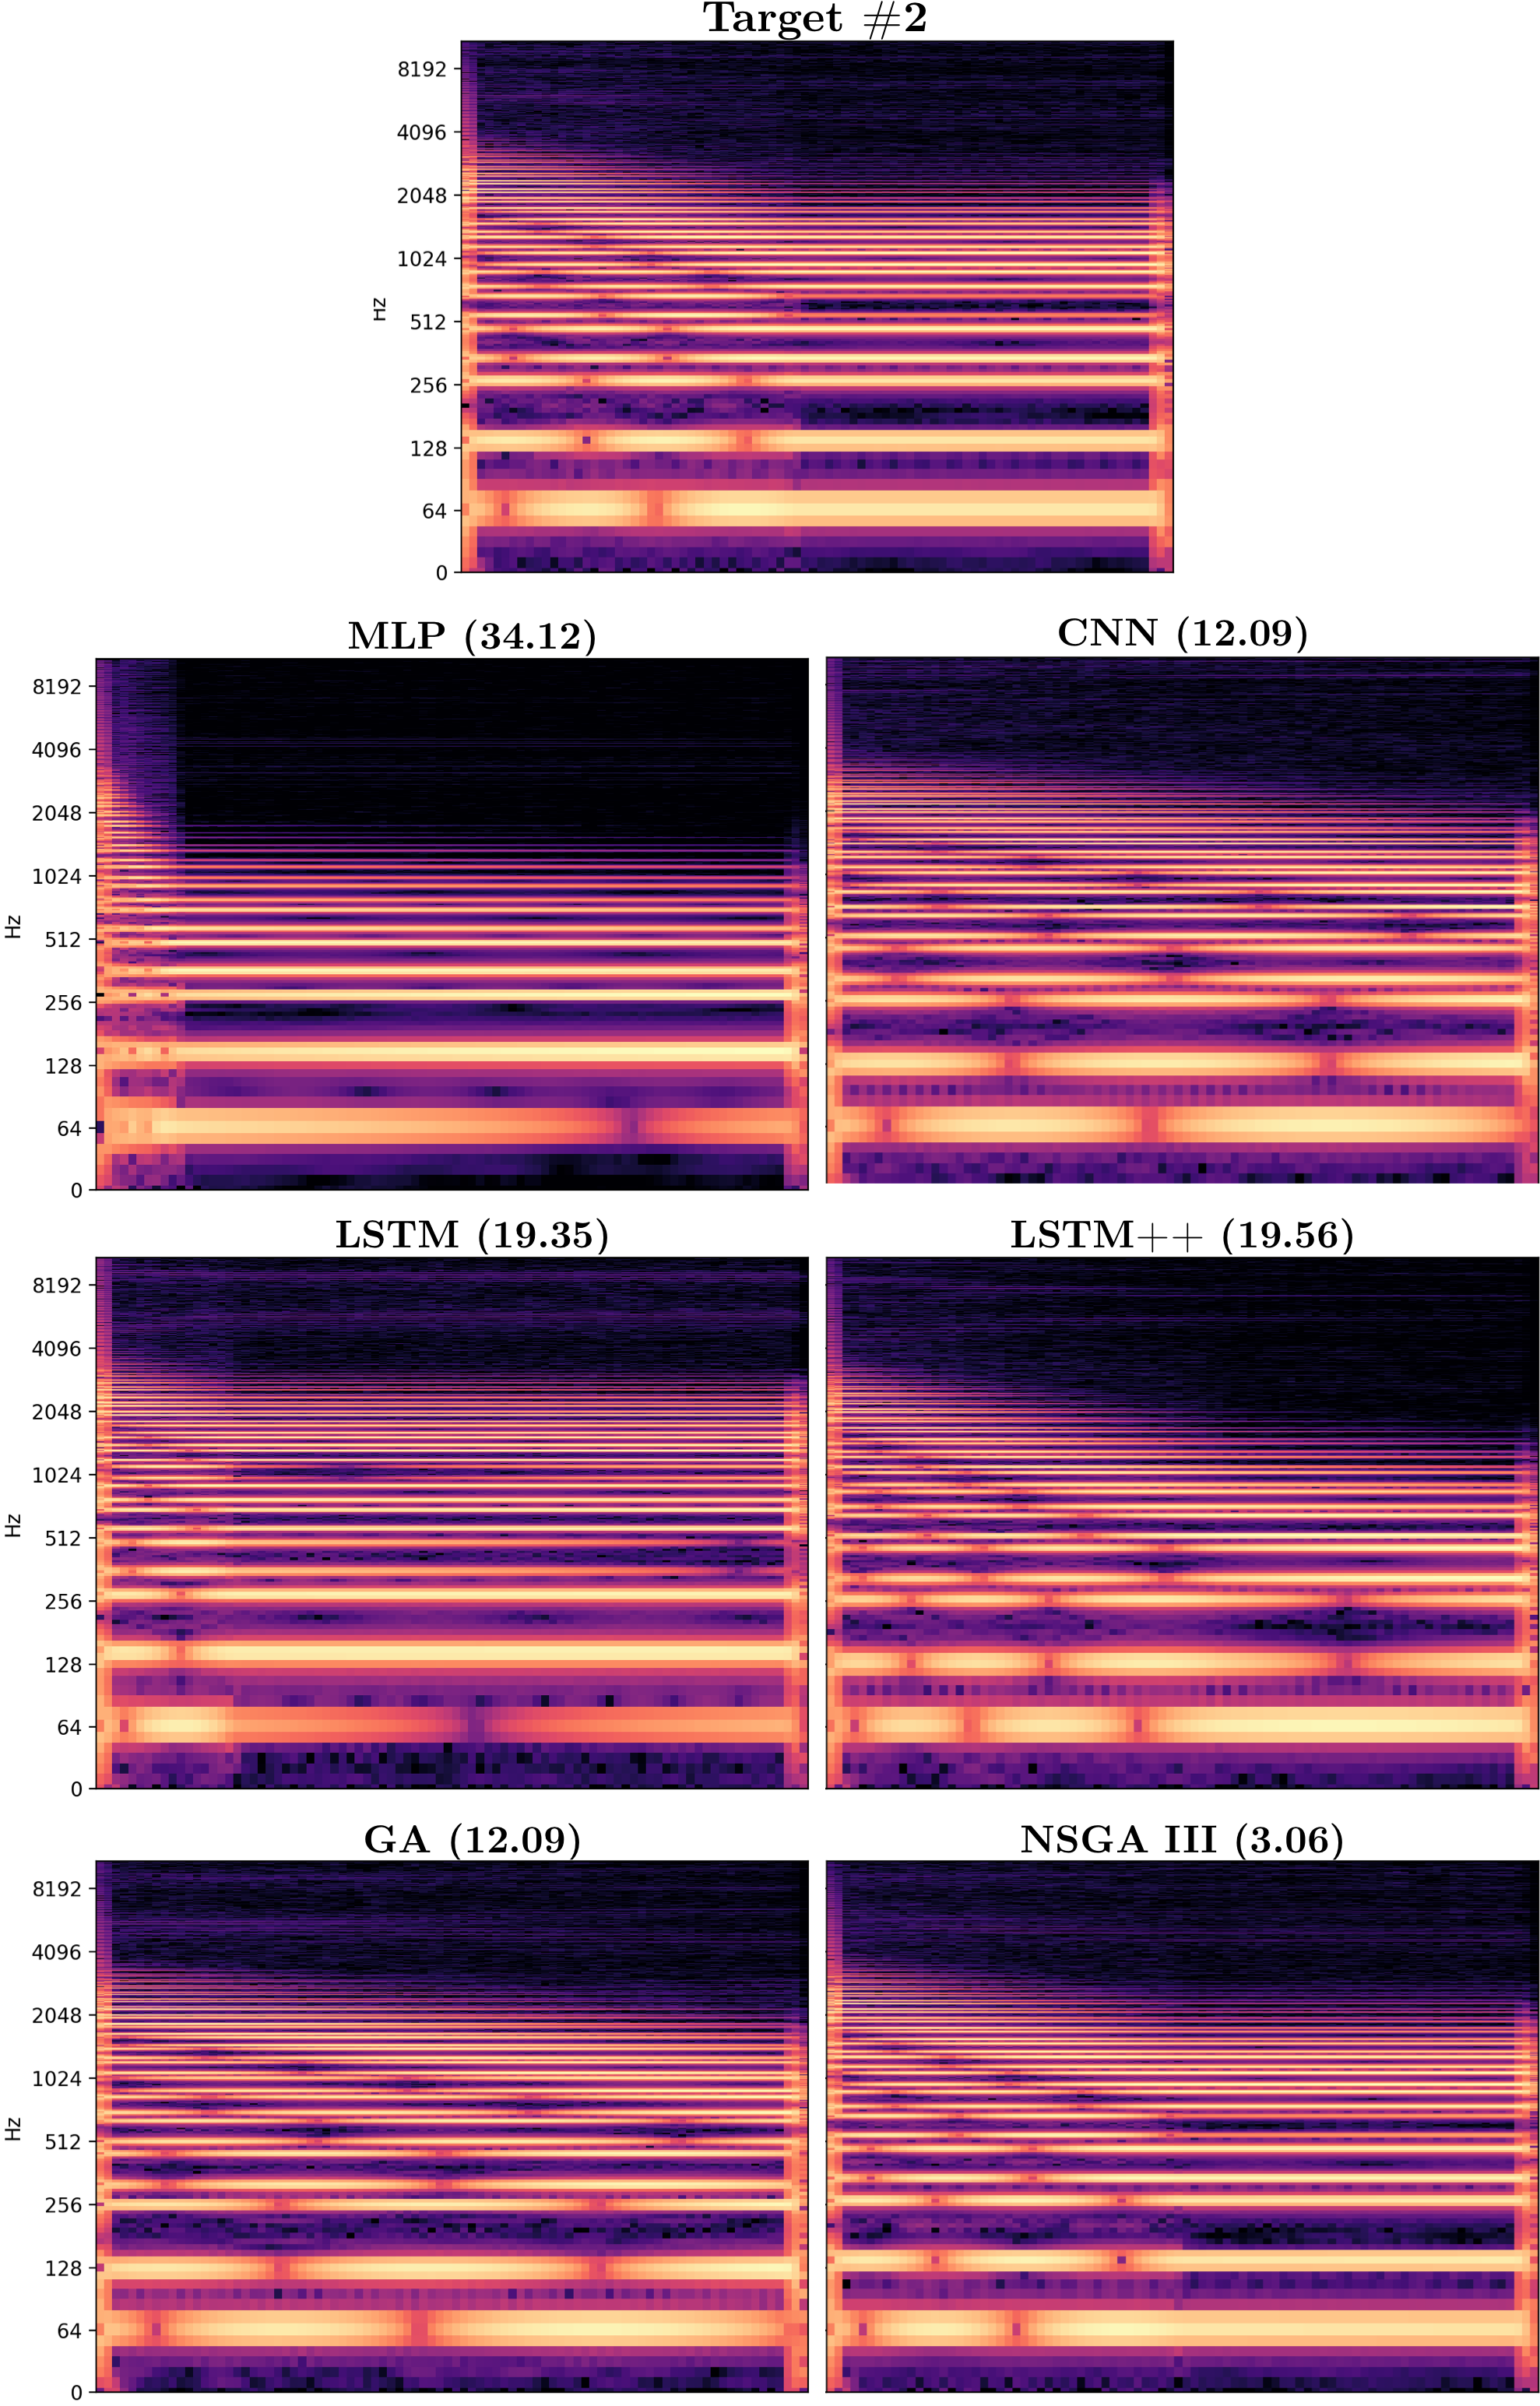
\includegraphics[width=0.75\textwidth]{spect_group_v1.png}
\caption{Spectrogram plots of a target sound and sound match predictions made by each estimator. The value next to the estimator name is the MAE value from MFCC evaluation for that prediction (lower MAE values indicate a closer match).}
\label{fig:group_spect}
\end{center}
\end{figure}

To evaluate to the resulting predictions the \mintinline{python}{MFCCEval} class was used, which calculates error and distance metrics on MFCCs of a target and prediction. Results for mean absolute error (MAE) which have been summarized using mean, standard deviation, minimum, and maximum, are shown for each estimator in table \ref{tbl:sound_match_eval}. Both GAs performed better than the deep learning approaches with the NSGA III having the best overall score. For deep learning approaches, the LSTM++ model achieved the best mean score. Histograms of the the MAE were also plotted for each estimator using the \mintinline{python}{plot_hist()} method in \mintinline{python}{EvaluationBase}. Histograms of the MAE for all predictions made by all estimators are shown in figure \ref{fig:group_hist}. Spectrograms of one target sound and sound match predictions made by each of the estimators for that target are shown in figure \ref{fig:group_spect}. For this particular target, spectrograms reveal that while the frequency and distribution of the harmonics was relatively close for each estimation, all estimators except for the NSGA III struggled with matching the temporal envelope of the spectrum.

% If we have time!!
%\subsection{Tunefish: Interactive Genetic}

\section{Future Work and Conclusion}
Development of \mintinline{python}{spiegelib} is ongoing and a number of expansions to the current library are planned. First, we would like to continue to expand the number of estimators available and plan on integrating the following: a hill climbing optimizer \cite{yee2018automatic}, a particle swarm optimizer \cite{heise2009automatic}, more 2D CNN configurations \cite{barkan2019inversynth}, a 1D CNN for raw audio input \cite{barkan2019inversynth}, and a generative approach \cite{esling2020flow}.  Second, we would like to expand on the type of interactions available such as automatic programming from vocal imitations \cite{mcartwright2014} and interactive methods. 
%Third, we would like to integrate more sophisticated subjective evaluation tools such as creating links to setup tests using the Web Audio Evaluation Tool \cite{waet2015}. Third, we would like to contribute to the $RenderMan$ library that is used in this work in order to extend support to Windows users and distribute the library via PyPI so the entire \mintinline{python}{spiegelib} library can be installed in one command. 
Finally, we would like to encourage developers and researchers from the automatic synthesizer programming community to contribute to \mintinline{python}{spiegelib}. Information on contributing is available online.\footnote{\url{https://spiegelib.github.io/spiegelib/contributing.html}} 

This work has introduced \mintinline{python}{spiegelib}, an open-source automatic synthesizer programming library. \mintinline{python}{spiegelib} is an object-oriented library that was designed with the goal of supporting development, collaboration, and reproducibility in the field. The library includes implementations of classes for conducting ASP research. These classes contain functionality for interacting with VST synthesizers, extracting audio features, creating datasets, estimating synthesizer parameters, and evaluating results. Six implementations of deep learning and evolutionary parameter estimation techniques based on previous work are included, with more planned. An example case of an automatic synthesizer sound matching study using the library was shown. This example case, along with the supporting code and data available online showcases how \mintinline{python}{spiegelib} can be used to support reproducible research.
